% Plot the stress versus strain curves for each test using the strain from the digital extensometer and the DIC calculations (i.e. two curves for each specimen).  Plot both stress vs strain curves for each specimen in the same plot.

In order to get an accurate idea of how these materials behaved and the mechanical properties of each layup, a stress vs. strain graph is a very useful tool. In this experiment the strain on each specimen was measured using two different methods, a digital image correlation (DIC) and the Instrom 2630-100 digital extensometer. This allowed for more accurate measurements to be taken and then compared once the experiment was finished. Although, there was an offset from between the DIC and extensometer, so that had to be corrected in the data before an accurate comparison could take place. With information on the strain, load, and size of each specimen, the following figures could be created for the $0\degree$, $45\degree$, and $90\degree$ laminates shown in Fig \ref{fig:stressvsstrain}.  One interesting to note from this is the behavior before breaking of all three tests. It can be seen in Fig \ref{fig:0lam} and Fig \ref{fig:90lam} that the stress is fairly linear until there is a sudden catastrophic failure with very little deformation of the material. This has to do with the orientation of the ply's within the composite, and when the are either parallel or perpendicular to the force, this type of behavior is to be expected. In Fig \ref{fig:45lam}, there is a linear region that translates to a more shallow slope until failure. This type of behavior occurs again due to the orientation of the laminates, with the load being distributed through both the matrix and fibers of the composite resulting in greater deformation and changes in the material property before failure. 

\begin{figure}[!h]
    \begin{center}
    \begin{subfigure}[b]{0.45\linewidth}
        \centering
        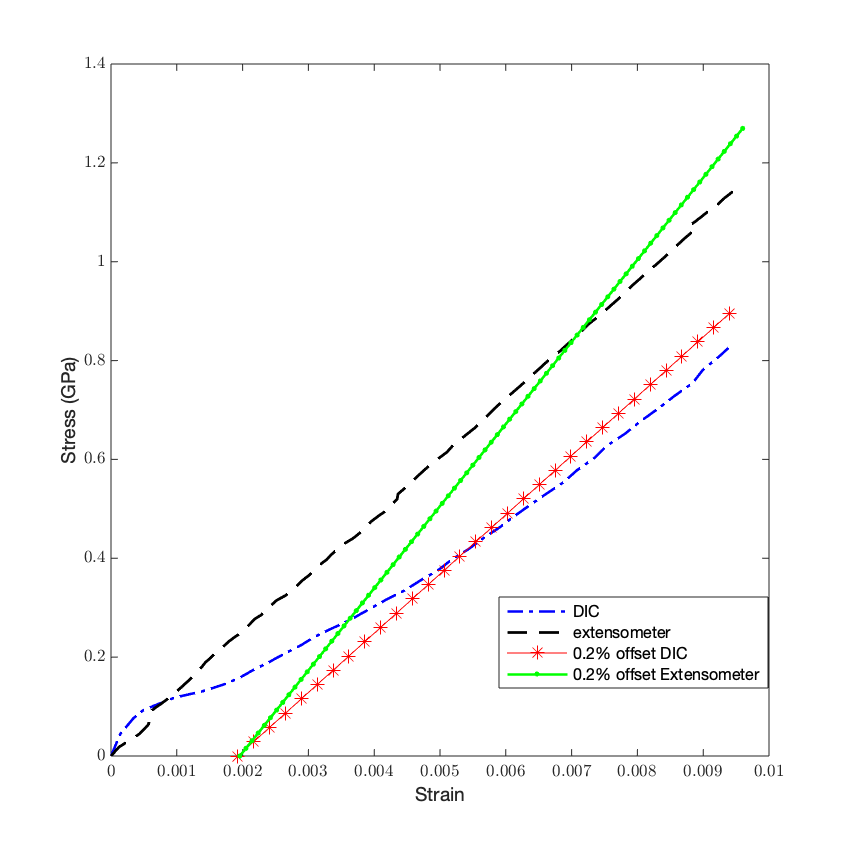
\includegraphics[width=\linewidth]{Pictures/stress vs strain/StressvsStrain_0.png}
        \caption{\textbf 0$\degree$ laminate}
        \label{fig:0lam}
    \end{subfigure}
    \begin{subfigure}[b]{0.45\linewidth}
        \centering
        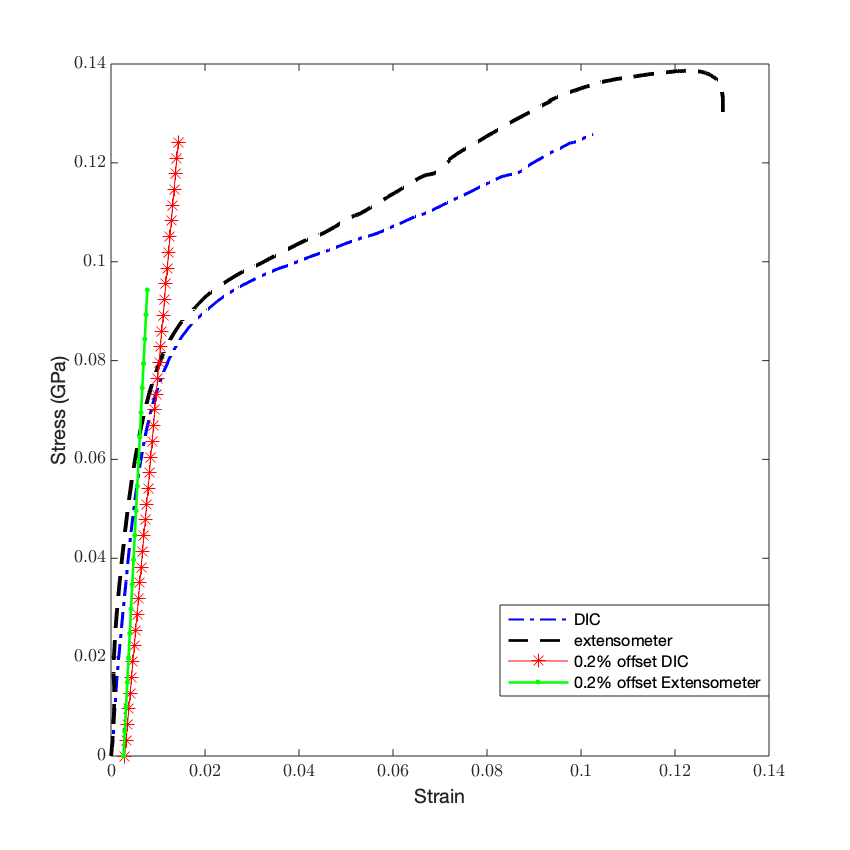
\includegraphics[width=\linewidth]{Pictures/stress vs strain/StressvsStrain_45.png}
        \caption{\textbf 45$\degree$ laminate}
        \label{fig:45lam}
    \end{subfigure}
    \end{center}
    \begin{center}
    \begin{subfigure}[b]{0.45\linewidth}
        \centering
        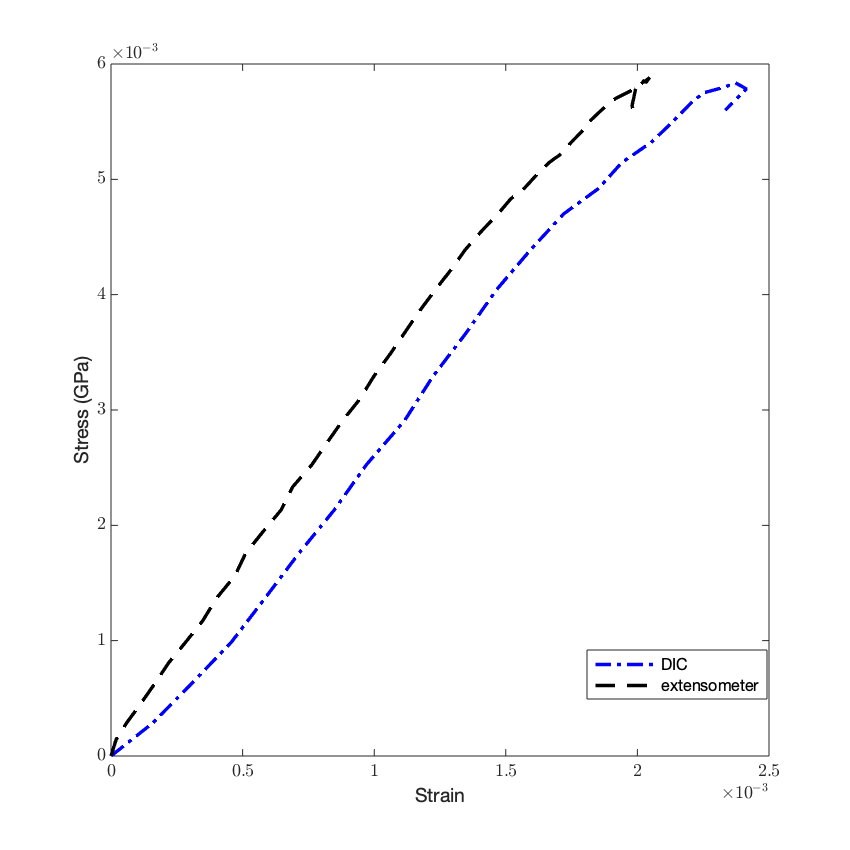
\includegraphics[width=\linewidth]{Pictures/stress vs strain/StressvsStrain_90.png}
        \caption{\textbf 90$\degree$ laminate}
        \label{fig:90lam}
    \end{subfigure}
    \end{center}
    \caption{Stress vs Strain plots comparing DIC to Extensometer measurements}
    \label{fig:stressvsstrain}
\end{figure}